\section{Earlier family, rule and delay diagnostics}\label{app:earlierdiagnostics}
\subsection{One-step rule diagnostics}
Across the seven default rules, adding native information generally improves efficiency,
but the effects are not orders of magnitude apart (Figure~\ref{fig:rules}). FACI-R with
residuals already gains 8.57\% and has lower coverage, while residual SAOCP overcovers
on average. CQR--PI-log, CQR--SF-OGD and CQR--ACI have similar average interval scores
but different local errors. SF-OGD has the smallest mean local error among these three
one-step CQR variants. A universal assertion that the score renders the rule irrelevant
is therefore unsupported even before adding delayed feedback.

\begin{figure}[htbp]\centering
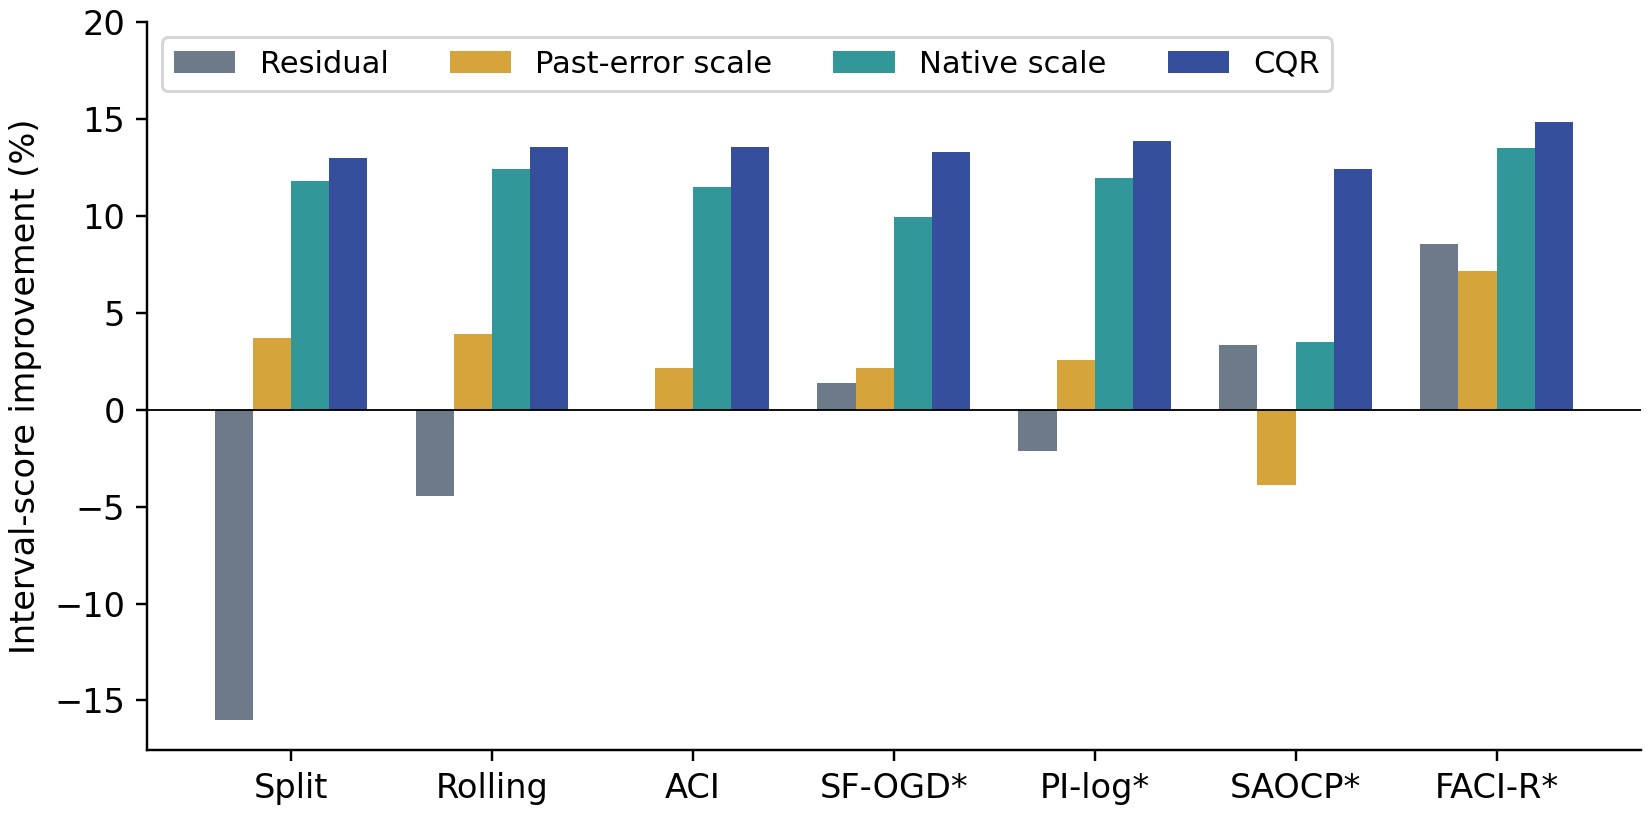
\includegraphics[width=\textwidth]{figures/score_rule.png}
\caption{Score--rule comparison on fixed one-step forecasts. Every gain uses the same
default residual--ACI denominator. Asterisks indicate the explicit adaptations described
in \ref{app:rules}; these labels do not claim equivalence to full original forecasting pipelines.}
\label{fig:rules}\end{figure}

\subsection{Benefits vary by family and persist on separate renewable series}
The mean CQR--ACI gain is 35.25\% on Alabama PV, 7.21\% on UCI loads, 5.96\% on ETT
and only 0.37\% on the three ERCOT loads (Table~\ref{tab:family}). The synthetic mean
is slightly negative. This heterogeneity is more informative than a pooled correlation
between a post-hoc volatility index and gains. Removing all eight PV series leaves
a 6.03\% gain, with descriptive interval $[4.25,7.88]\%$. Restricting to the 25 observed
series yields 15.16\%; that subset gives PV a larger relative weight. Leave-one-family-out
means remain positive, ranging from 6.03\% to 16.60\%.

\begin{table}[htbp]\centering\small
\caption{CQR--ACI gains by main-panel family. Intervals resample series within the listed
family and are descriptive; narrow intervals for correlated PV plants do not imply broad
geographic certainty. Small two- or three-series groups have especially limited precision.}
\label{tab:family}\begin{tabular}{lrrr}
\toprule
Family & Series & Gain (\%) & Descriptive 95\% CI \\
\midrule
Alabama PV & 8 & 35.25 & [34.75, 35.74] \\
Constructed seasons & 2 & 8.58 & [6.25, 10.90] \\
Constructed switches & 2 & 12.31 & [11.36, 13.27] \\
ERCOT & 3 & 0.37 & [-1.53, 1.86] \\
ETT & 4 & 5.96 & [3.41, 8.51] \\
Synthetic & 2 & -0.05 & [-0.42, 0.31] \\
UCI load & 10 & 7.21 & [5.53, 9.70] \\
\bottomrule
\end{tabular}
\end{table}
\begin{figure}[htbp]\centering
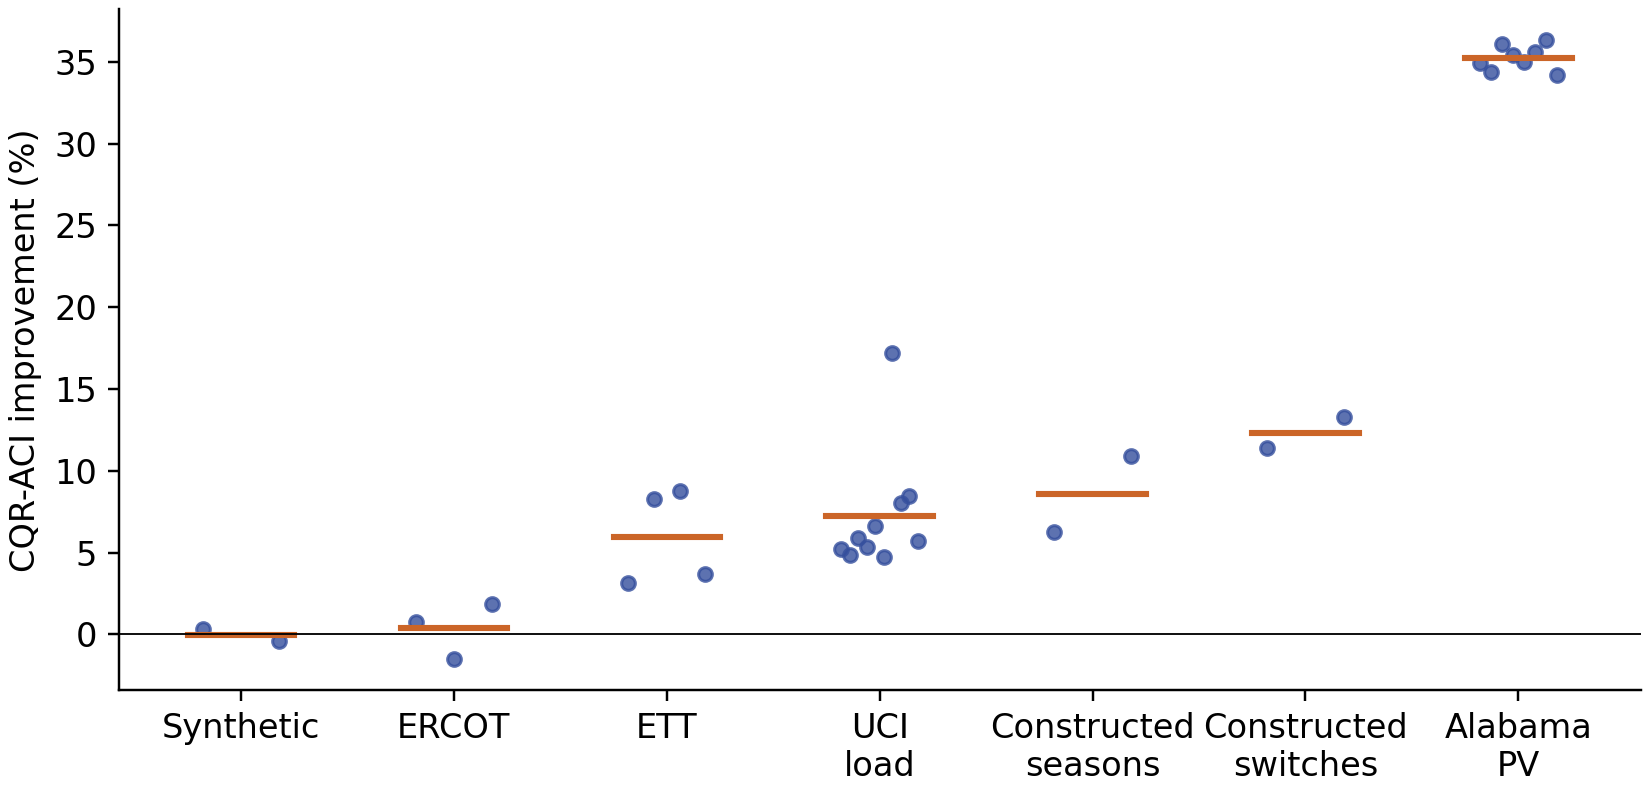
\includegraphics[width=\textwidth]{figures/families.png}
\caption{Each point is one series averaged across four backbones; horizontal orange marks
are family means. Constructed and synthetic series remain visible rather than being
counted as independent observed energy systems.}\label{fig:families}\end{figure}

Per-backbone mean gains are 15.15\% for Chronos-2, 13.82\% for Chronos-Bolt, 12.90\%
for Moirai and 12.41\% for the archived TimesFM configuration. On the separate GEFCom
panel, CQR--ACI gains 19.63\% overall: 41.46\% for solar and 13.08\% for wind, with
89.99\% mean coverage. This is evidence beyond the Alabama solar panel, but does not
convert correlated zones into independent geographic samples.

At block lengths 100, 200 and 400, 109 primary pairs have a positive paired-bootstrap
95\% interval and two have a negative interval. The centered-test/BH procedure identifies
109 positive and two negative differences at each of these block lengths. These counts
are reported with the dependence caveat above; the magnitude and family distribution of
the effect remain the main empirical evidence.

\subsection{Delayed feedback makes rule choice consequential}
Figure~\ref{fig:horizon} and Table~\ref{tab:horizon} show the joint horizon/feedback
experiment. At $h=24$, CQR--ACI has 87.34\% mean coverage, compared with 87.10\% for
residual--ACI. CQR--PI-log attains 89.96\% coverage and a 17.09\% score improvement
relative to residual--ACI, compared with 13.15\% for CQR--ACI. CQR--ACI's average number
of clipped updates, counting validation and test adaptation, increases from 3.06 at
$h=1$ to 201 at $h=24$. This is consistent with the projection term in
Equation~\eqref{eq:identity}, although a count alone does not measure its signed magnitude.

\begin{figure}[htbp]\centering
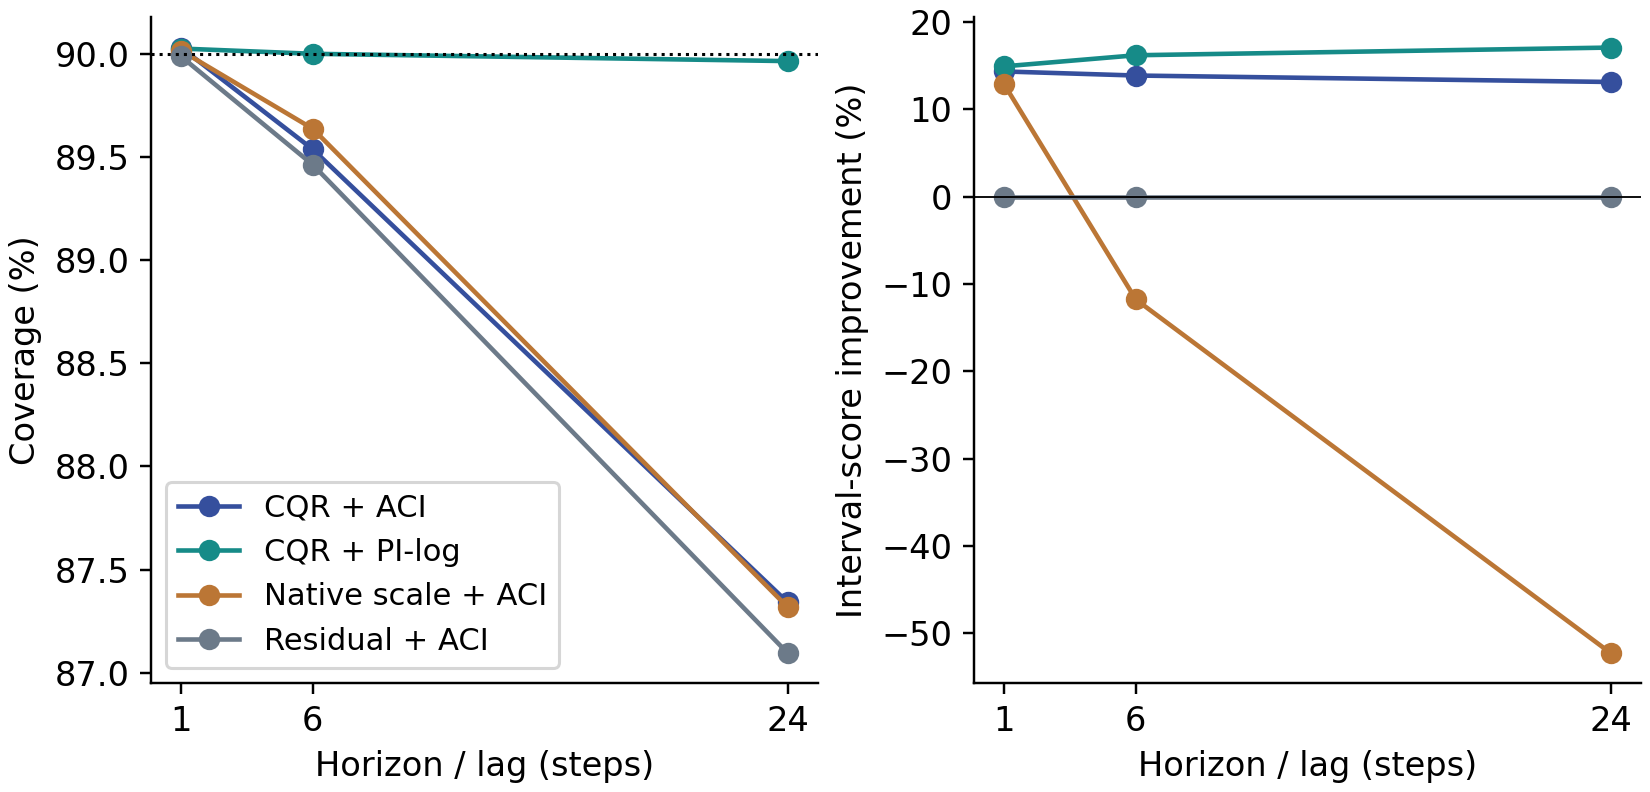
\includegraphics[width=\textwidth]{figures/horizon.png}
\caption{Joint changes in horizon and natural feedback delay on eight series and two
Chronos models. Coverage is an average; score gains use the horizon-specific residual--ACI
denominator. Solar steps are ten minutes, so $h=24$ is not day-ahead for those series.}
\label{fig:horizon}\end{figure}

The PI result is not a claim of uniformly improved reliability. At $h=24$, its local
150-origin coverage error is 4.86 percentage points, versus 4.52 for CQR--ACI. Improved
overall coverage can coexist with worse local variation. The controller also emits some
singletons after negative signed corrections: CQR--PI-log's average singleton rate is
0.567\% at $h=24$, versus 0.048\% for CQR--ACI. No infinite test intervals occur for
these two reported variants in this panel.

The fixed-forecast intervention separates lag from changing forecast difficulty
(Figure~\ref{fig:delay}). On the same $h=1$ predictions, increasing calibration lag from
1 to 24 steps changes residual--ACI coverage from 89.99\% to 88.62\% and CQR--ACI from
90.03\% to 89.52\%. CQR--PI-log remains at 89.99\% for lag 24, while its local coverage
error is 2.88 percentage points compared with 2.08 for CQR--ACI. Thus feedback restriction
alone can alter the relevant coverage comparison. The larger deficit in true $h=24$
forecasts additionally reflects changes in the forecast/score stream; lag alone does not
explain its entire magnitude.

\begin{figure}[htbp]\centering
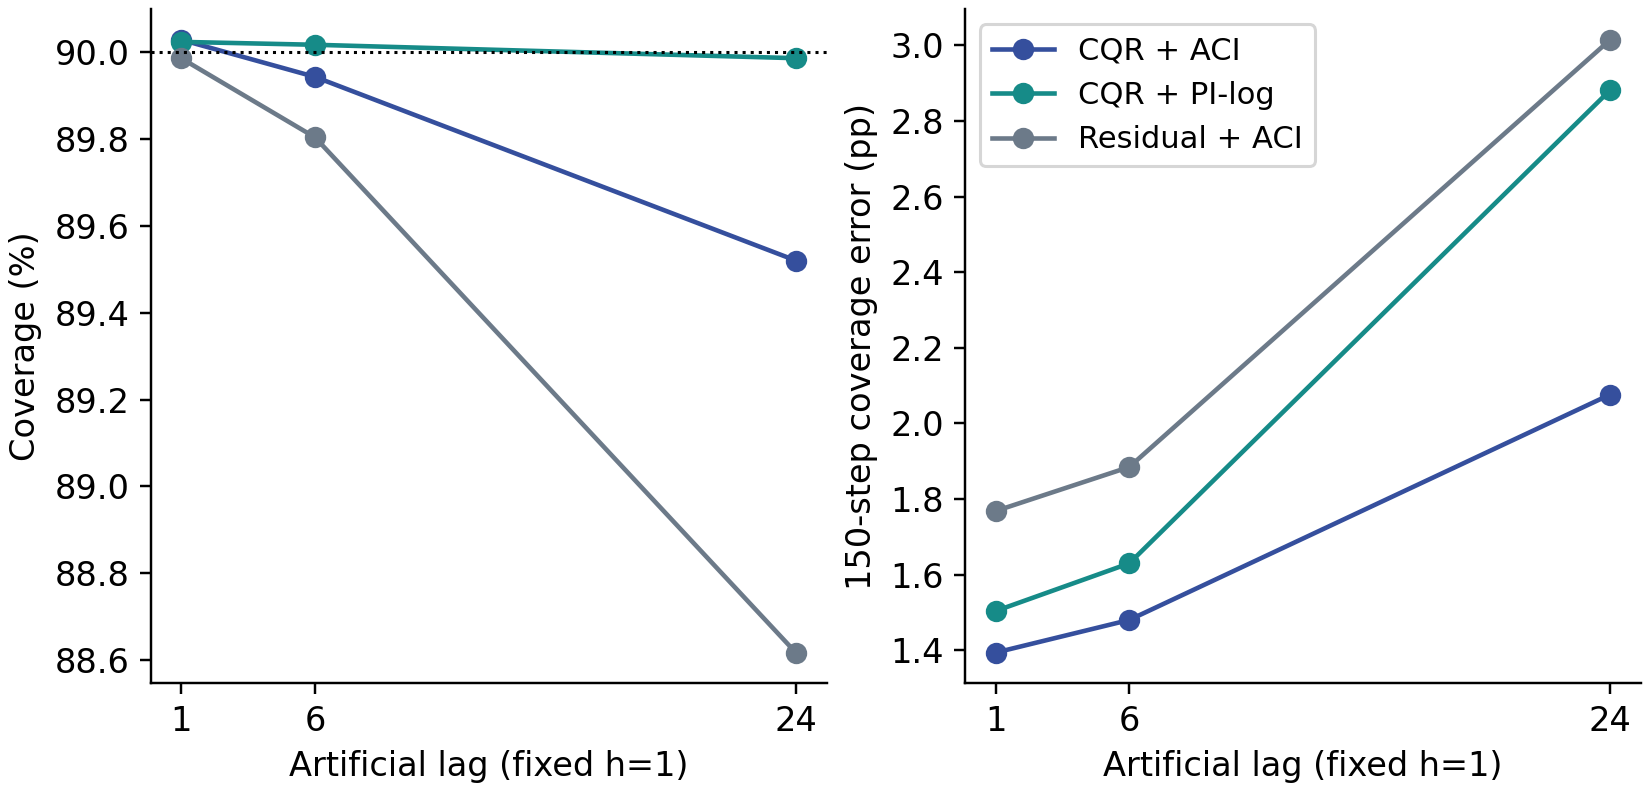
\includegraphics[width=\textwidth]{figures/delay_control.png}
\caption{Exploratory intervention holding one-step predictions and targets fixed while
withholding calibration outcomes. Overall coverage and local coverage error respond
differently. This isolates the calibrator's feedback channel, not the model's context.}
\label{fig:delay}\end{figure}

\subsection{Earlier long-horizon PV diagnostics}
The separate long-horizon diagnostic concerns two other development photovoltaic
series and two backbones, so it is not a within-panel comparison with the one-step
decomposition.
On the two development photovoltaic series and two backbones, tuned CQR--COP at
$h=24$ attains 90.41\% overall coverage, yet only 79.93\% on positive-output targets
and 97.05\% on zero-output targets (Figure~\ref{fig:solarconditional}). Zero outputs
constitute approximately 61.04\% of these test segments. At $h=1$ and $h=6$,
positive-output coverage is 87.95\% and 82.42\%, respectively, despite overall coverage
near 90\%. These are four model--series pairs from two series, not four independent
solar datasets. Positive output is an outcome-defined diagnostic and need not
coincide with astronomical daytime. A marginal coverage theorem does not promise
coverage on this subset, so the finding is not a counterexample to that theorem.

\begin{figure}[!htbp]\centering
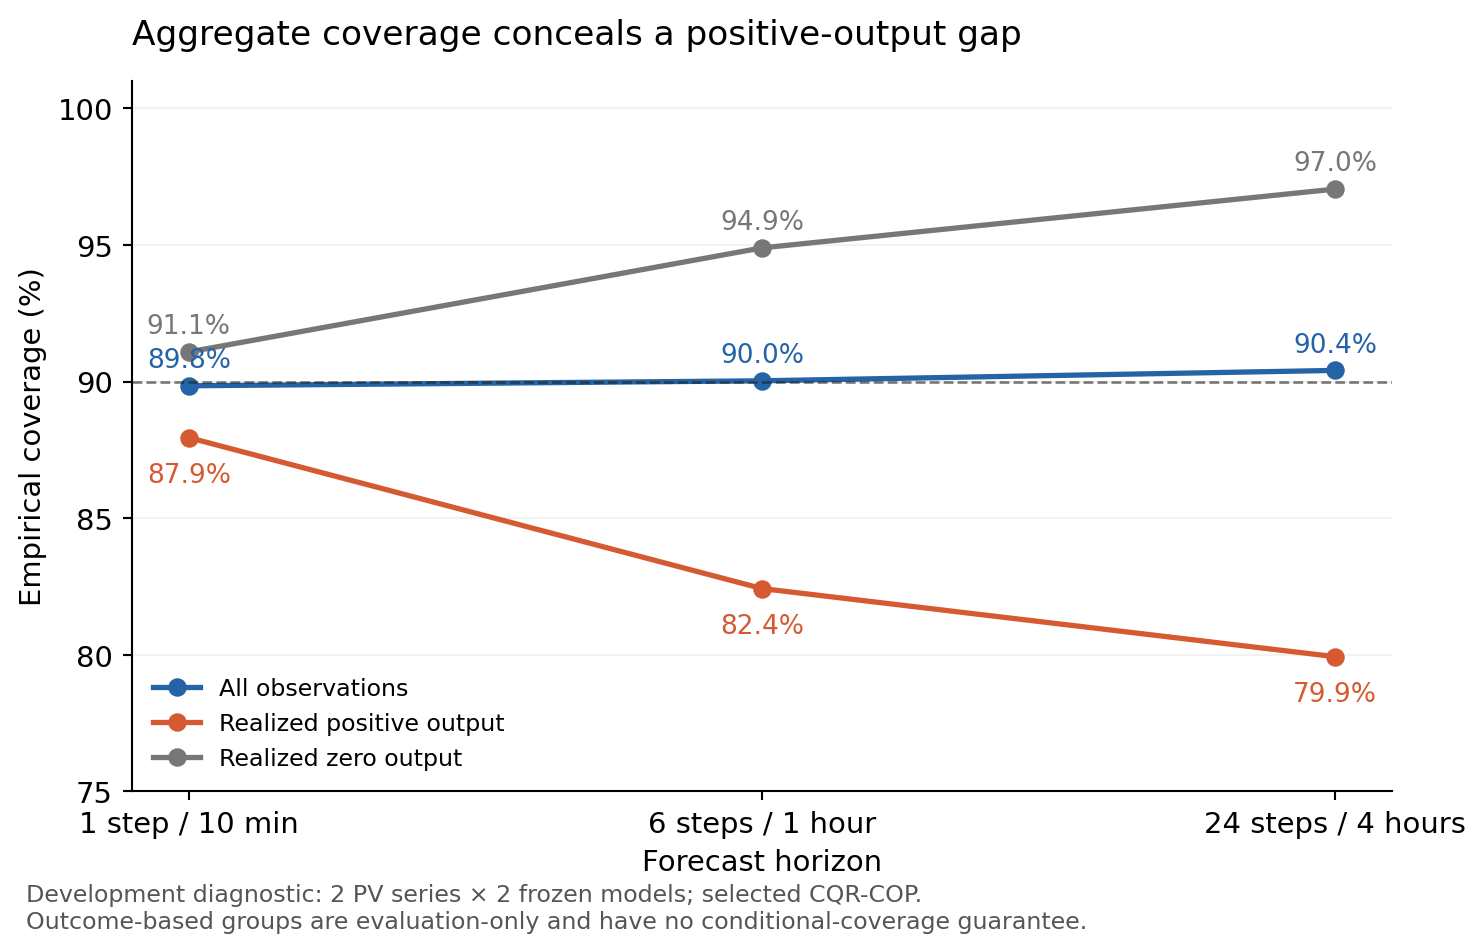
\includegraphics[width=\textwidth]{figures/solar_conditional_coverage.png}
\caption{Post-hoc photovoltaic reliability diagnostic for selected CQR--COP.
Coverages average over two series and two models. The zero/positive labels are used
only for evaluation; prediction and validation never use the future target label.
At this sampling rate, 24 steps represent four hours.}
\label{fig:solarconditional}\end{figure}

The observable-width grouping experiment tests whether a simple existing approach
can reduce the deficit. Separating both memory and state increases positive-output
coverage from 78.93\% to 83.49\% relative to matched shared-state CQR on these solar
pairs. Overall coverage changes from 88.46\% to 89.45\%, with a 2.47\% interval-score
gain. The positive-output gap remains substantial. Separating memory alone improves
solar interval score by 6.75\% but reduces overall coverage to 85.66\%, illustrating
why a proper-score change should be accompanied by coverage diagnostics.
Across all 16 development pairs, the both-grouped CQR gain is only 1.12\%.
On the confirmation families, the same grouping yields a 3.27\% gain at $h=24$,
but coverage remains 88.56\%, compared with 87.87\% for shared ACI. Grouping is thus
an informative control, not a demonstrated solution to conditional reliability.

